\documentclass[a4paper, 10pt, titlepage, twocolumn, onehalfspace]{article}



\usepackage{apacite}
\usepackage{simpleConference}
\usepackage{times}
\usepackage{apacite}
\usepackage{graphicx}
\usepackage{amssymb}
\usepackage{url}
\usepackage{xcolor}
\usepackage{alltt}
\usepackage{tikz}
\usepackage{ulem}
\usepackage{setspace}
\usetikzlibrary{trees}


\newcommand
{\image}[2]{\vspace{10 mm} \includegraphics[width=\textwidth]{#1}
\begin{center} \caption{#2} \end{center}
\vspace{10 mm}
}

\definecolor{light-gray}{gray}{0.95}
% Compensate for fbox sep:
\newcommand\Hi[2][light-gray]{%
  \hspace*{-\fboxsep}%
  \colorbox{#1}{#2}%
  \hspace*{-\fboxsep}%
}

% Command for inserting a todo item
%http://midtiby.blogspot.ie/2007/09/todo-notes-in-latex.html
\newcommand{\todo}[1]{%
% Add to todo list
\addcontentsline{tdo}{todo}{\protect{#1}}%
%
\begin{tikzpicture}[remember picture, baseline=-0.75ex]%
\node [coordinate] (inText) {};
\end{tikzpicture}%
%
% Make the margin par
\marginpar{%
\begin{tikzpicture}[remember picture]%
\definecolor{orange}{rgb}{1,0.5,0}
\draw node[draw=black, fill=orange, text width = 3cm] (inNote)
{#1};%
\end{tikzpicture}%
}%
%
\begin{tikzpicture}[remember picture, overlay]%
\draw[draw = orange, thick]
([yshift=-0.2cm] inText)
-| ([xshift=-0.2cm] inNote.west)
-| (inNote.west);
\end{tikzpicture}%
%
}%



\begin{document}


\title{Implementing a Horizontal Size of KDGEs Information Classification and Visualization System}
\author{Steven Diviney \\
08462267
}


\maketitle

\newpage

\begin{abstract}
This article discusses the field of Information Visualization. My research project is discussed briefly to provide context, but the bulk of the text deals directly with the field of Information Visualization. First it is defined. A brief summary of its history is then given followed by my attempt to explain how a visualization helps accelerate cognition and the challenges encountered in attempting to do so. Some well established methods of visualization are then briefly presented and analyzed. Finlay evaluation criteria for the project are defined. 
\end{abstract}


\section{Introduction}
Information visualization is defined as an internal construction in the mind. The field of Information Visualization is concerned with creating visual artifacts in order to facilitate individuals in building an internal representation of a dataset \cite{spence2001information}. In this paper the term visualization refers to the creation of these visual artifacts unless explicitly stated as the cognitive process of understanding an image.

There are three fields subfields of Information Visualization. The boundaries between them are not particularly distinct and they are referred to somewhat interchangeably in academic literature. There are many other types but these three are of particular interest as their primary concern is the visualization of large volumes of data almost always with the aid of a computer.
\subsection{Information Visualization}
Information visualization is perhaps the most broadly used and can be thought to encompass all of the fields of visualization. After all, almost anything if sufficiently organized, is information of a sort \cite{friendly2001milestones}. Friendly notes that tables, graphs, maps and even text, whether static or dynamic, provide some means to see what lies within, determine the answer to a question, find relations, and perhaps apprehend things which could not be seen so readily in other forms. 

The term today is generally applied to the visual representation of large-scale collections of non-numerical information, such as text in a book or files on a hard-disk. The distinction between this definition and that of Data Visualization seems to be quite poor. The type of the data in question is used to distinguish the two. The terms ``information" and ``data" are not so easily distinguished. Information can be thought of as a level of abstraction above data. The mere fact that a dataset is non-numerical does not identify it as information. A set of ordinal labels or categories is just as meaningless as a set of numbers. Information is created by organizing such data and presenting it with context.

Information visualization is concerned with representing more abstract topics. A good example is process visualization. Each element in a process visualization represents a complex topic.

\subsection{Data Visualization}
Data Visualization is the science of visual representation of data, defined as ``facts and statistics collected together for reference or analysis" \cite{oed31}. As stated the distinction between data and Information Visualization is not very concrete. In researching for this paper I have come across several examples of one labeled as the other. As far as I can tell there have been no calls to address this issue and the two are used interchangeably to a large extent.

Interestingly the majority of literature I have come across states it is concerned with Information Visualization, and then goes on to outline steps to transform data into a visual artifact in order to help the synthesis of information. From this it would seem quite clear that the distinction is not regarded as important but I would like to point out my topic of study is concerned with Data Visualization. The synthesis of new information through the creation of visual artifacts.

\subsection{Scientific Visualization}
Fortunately Scientific Visualization is very well defined. It is concerned primarily with the visualization of objects in three dimensional space with an emphasis on realistic rendering. This emphasis on realism is primarily what distinguishes it from other forms of visualization. This is not to say that the other forms may distort the data, rather that abstract data does not necessarily have a spatial dimension. How would one realistically visualize the lines of a book? Novel ways must be invented to accomplish this.

\subsection{KDEG's Information and Visualization System}
KDEG, the Knowledge and Data Engineering Group in Trinity College Dublin are developing a system to automate the process of Data Visualization. The creation of a visualization is typically quite a manual process. There are an abundance of tools that, given a dataset, produce specific types of visualizations. These tools expect the data to be formatted in a certain way and for the user to manually specify certain attributes of the data to the visualization tool. They also require a domain expert to contribute some knowledge about the nature of the data in order to create information. Typically the domain expert requires the assistance of a knowledge engineer to encode this knowledge into a format a machine can use \cite{champ}.

KDEG are attempting to build a system that can take data from multiplier sources, classify it, determine the form of the data and associate it with appropriate visualizations. Information about the data can be added by a domain expert without the aid of a knowledge engineer. What they lack at the moment is a method to take this data and associate it with appropriate visualizations.

My task is to implement a complete horizontal slice of this system. Given a dataset that has been augmented with expert knowledge my system must determine the nature of the data to represent, its dimensionality, the data structures needed and associate it with an appropriate visualization. The input data has been restricted to few sets that share certain attributes. Implementing a compete system is not feasible in the time frame. The goal of developing such a system is to document the process of Data Visualization which is poorly understood. The steps outlines above, determining dimensionality, data structures etc. are sometimes done automatically in certain cases but are typically linked together manually. An overview of the steps needed to create a visualization is presented below.

\subsection{Visualization Synthesis}
The creation of a visual artifact follows three successive stages \cite{mazza2009introduction}. These steps are by no means definitive. One of the major problems within the field of Data Visualization is the lack of consensus on a single process. Most of what I found during my research is some variation of the following;

\begin{itemize}
\item Preprocessing and data transformations.
\item Visual mapping.
\item View creation.
\end{itemize}

\subsubsection{Preprocessing and data transformations}
The initial phase is concerned with taking raw data, that is data supplied by the world, or datasets, and organizing them them into a logical structure suitable for machine processing. Additional information can be added in this preliminary step. Filtering operations can be used to eliminate unnecessary data and calculations can be used to obtain new data, i.e. the summation of particular record instances.
\subsubsection{Visual mapping}
This stage determines the form of the data. Again, abstract data does not always have a location in physical space associated with it, so a visual mapping is needed. Mazza notes ``The spatial substrate defines the dimensions in physical space where this visual representation is created" \cite{mazza2009introduction}. It is defined in terms of axis. The nature of the data determines this mapping. Quantitative, ordinal and nominal data are all reported in different ways along an axis. The graphical elements used to display the data and their properties are also defined at this stage.
\subsubsection{View creation}
The view renders the visual representation on the display of the computer. The main issue here arises when the quantity of data is too large for the display. There is a large body of research surrounding this problem as it is very common. My thesis will attempt to tackle some of these issues. In order to utilize the available screen space efficiently the data must be rendered in order of importance. This will be explained further in a later section.


\section{History of Visualization}
Visualization is one of the oldest fields of human inquiry. The earliest examples are of geometric diagrams and maps to aid navigation. The earliest known map is generally regarded to be a map of ``Konya", a town in Turkey, dating back to 6200BC \cite{bagrow2009history}. Humans have perhaps been using graphical representation of the world around them to convey information for far longer, up to 14,000 years ago \cite{caves}. Diagrams used to illustrate concepts rather than spatial features did not appear until much later.

Visualization has only recently become a field in its own right. Up until recently it was simply a tool used to convey data. As such it had to wait for advancements in other fields to progress. The 16th century saw significant advancement in the techniques and instruments used for precise observation and measurement of physical quantities. Astronomers, surveyors and cartographers needed to convey greater amounts of increasingly precise information. The field of mathematics was also seeing the birth of probability theory, analytic geometry and theories of estimation and measurement.

The 19th century saw an explosion of statistical graphics \cite{friendly2001milestones}. Bar charts, histograms, line graphs. Statistics was becoming an increasingly important field and began to see use in social planning, commerce, transportation and other areas. For the first time visualization was used to explain data rather than just supplement its description with an illustration. This was the first revolution in the field of visualization. Up until the 19th century visualization was simply a tool, used and developed as the need arose.

One of the most famous examples of the use of visualization to convey an idea is the dot map used to illustrate the source of a cholera epidemic in London, Figure ~\ref{fig:dot_map}. John Snow, an English physician theorized that cholera was spreading through the cities water supply, not the air as was accepted at the time. Snow's chemical examinations of the water from the Broad Street pump were not sufficient to prove it as the source. Rather his studies of the pattern of the disease were what convinced the local authorities. He plotted each case of cholera on a map. The map clearly shows the water pump at the center of the outbreak \cite{frerichs2007ghost}.


\begin{figure*}[hbt]
  \begin{center}
    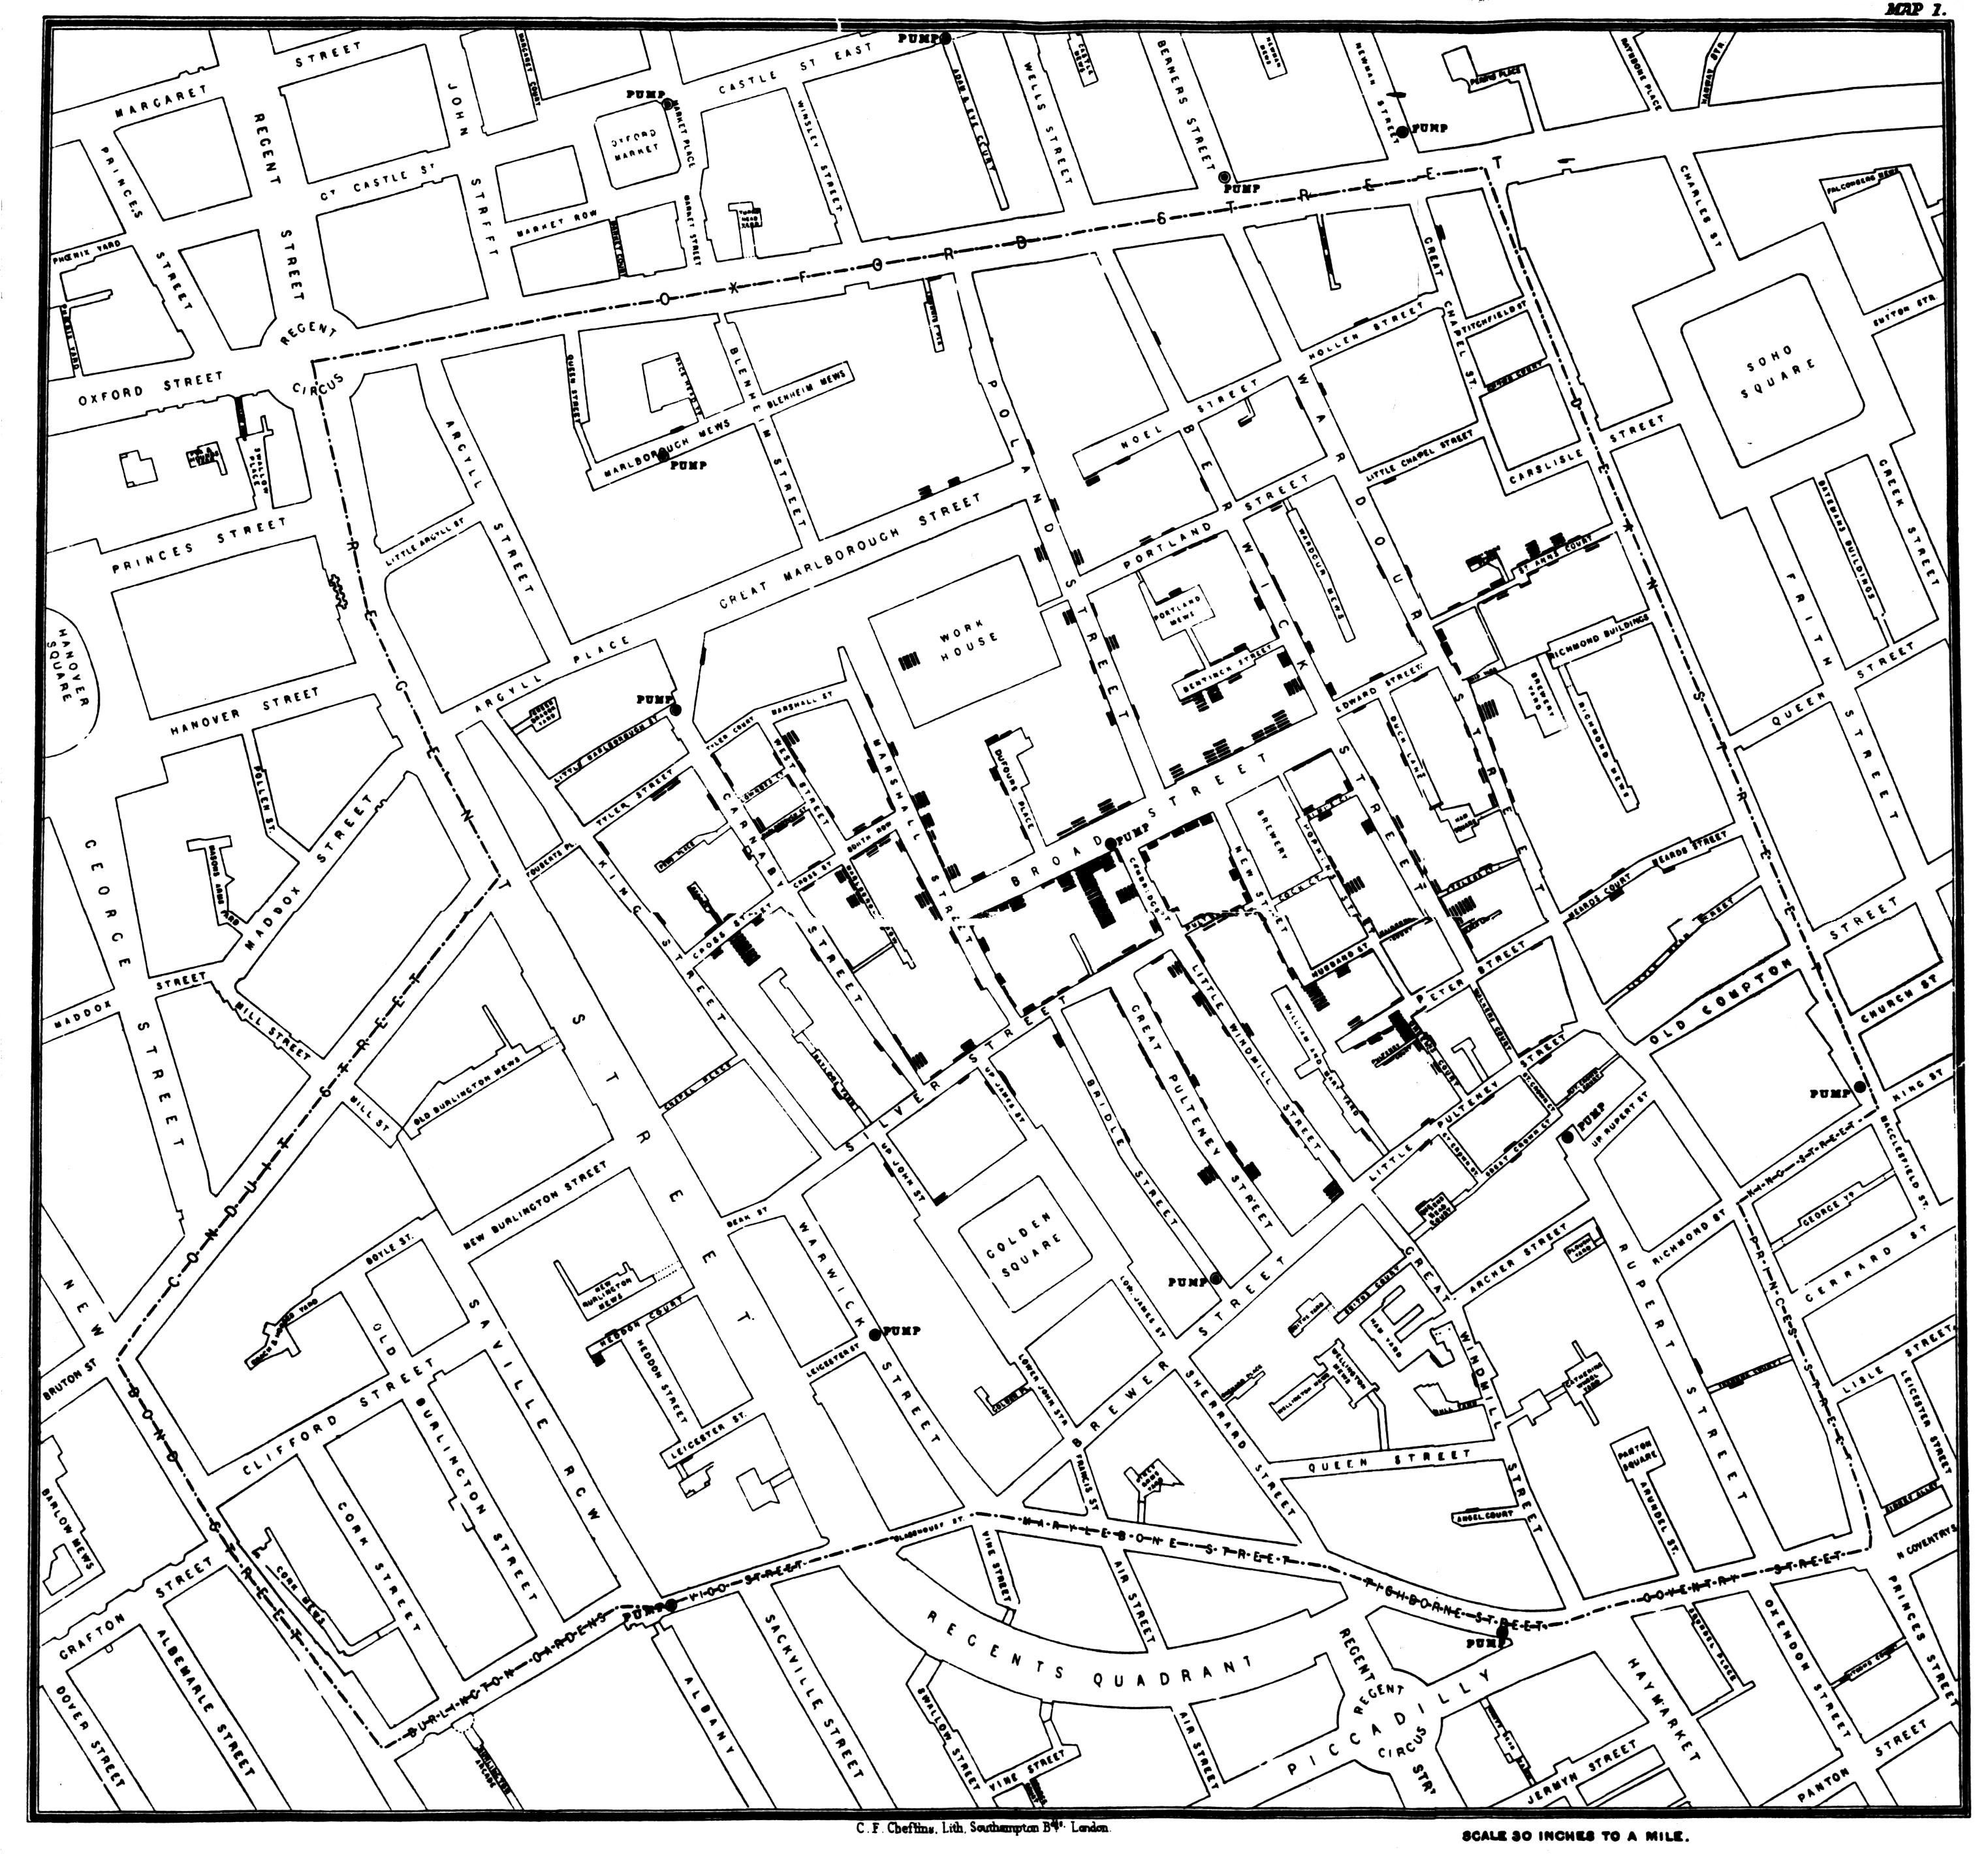
\includegraphics[width=3.5in]{snow.jpg}
  \end{center}
  \caption{\small Dot map showing cholera cases per household. }
  \label{fig:dot_map}
\end{figure*}


\begin{figure*}[hbt]
  \begin{center}
    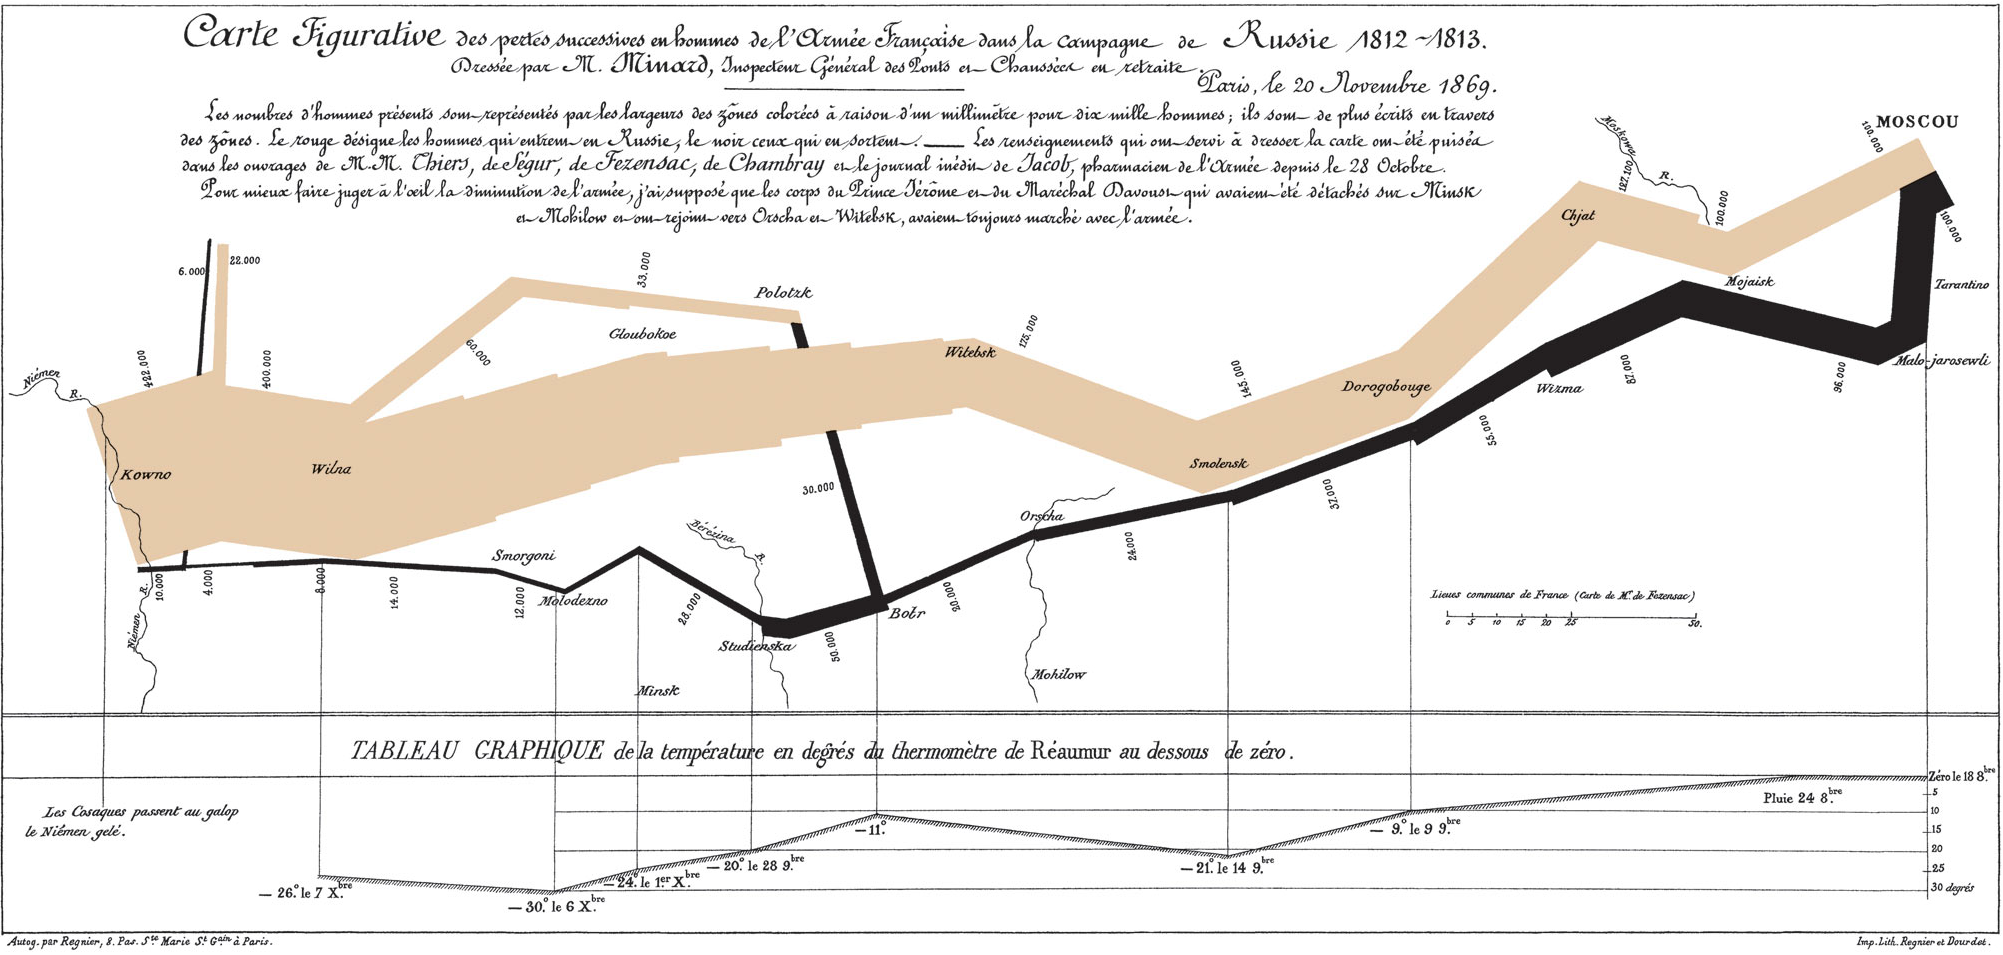
\includegraphics[width=3.5in]{Minard.png}
  \end{center}
  \caption{\small Napoleon's march on Moscow.}
  \label{fig:march}
\end{figure*}



Visualization is a field heavily intertwined with human psychology. This will be examined later in greater detail but I draw attention to it here to illustrate just how concise an effective visualization can be. Human perception, particularity visual perception, is a very complex process. However certain visual attributes, such as size or colour, are given perceptual preference. They are what we focus on and process first \cite{mackinlay1986automating}. A visualization that exploits this fact effectively is arguably far more effective than any textual description. Charles Minard's flow map of Napoleon's march to Russia, Figure ~\ref{fig::march} is perhaps one of the most famous visualizations ever created, shown again and again in academic literature. The graphic conveys several pieces of complex information at once. The size of the army corresponds to the width of the line and is the most obvious feature. It provides a strong representation of the human suffering. Rivers along the route can be identified by a sudden loss of life. The line shows the direction and route the army took. The date and temperature are also recorded along the path.

The 19th century has been called the ``Golden Age of Statistical Graphics" \cite{friendly2008golden}. Progress in the field slowed around the turn of the 20th century. Statisticians had begun to regard pictures incapable of stating fact, at least with no where near the precision as their new statistical models \cite{friendly2000discussion}. Several attempts were made to compare the relative effectiveness of various visualizations but the conclusions of these early experiments were inconclusive and contradictory \cite{fienberg1979graphical}. There is also a definite drop in the number of publications in the field around the first half of the 20th century. In 1915 The American Society of Mechanical Engineers published 17 basic rules of elementary graphic presentation. A publication by such a body is somewhat telling. Visualization had once again become a tool. The golden age had yielded a wide array of visualizations. Graphical methods began to enter textbooks, saw use in government, education, commerce and science \cite{haskell1919make,ayres1919war,gantt1919organization}. Although publications surrounding visualizations had stagnated their usage had reached its peak \cite{fienberg1979graphical}.

\subsection{Modern Visualization}

From 1950 to 1970 Information Visualization underwent a seismic shift, spurred by three developments \cite{friendly2001milestones};
\begin{itemize}
\item ``The Future of Data Analysis" issued a call for the recognition of data analysis as a legitimate branch of statistics \cite{tukey1962future}
\item ``Semiologie Graphique" \cite{bertin1973semiologie} organized visual and perceptual components of graphics according to their features and relations between data. It is widely regarded as the ``periodic table" of Information Visualization. It outlined the primitives of any visualization.
\item Computer processing of data had begun. It offered the opportunity to create new graphical forms and processes quantities of data that had before been unpractical.
\end{itemize}

The 1970s saw the beginning of the computer revolution. Visualization saw a large increase in both usage and research. The computer allowed vast quantities of information to be processed and higher dimensionality visualizations began to emerge such as the scatter-plot. Human psychology began to be employed in creating more effective visualizations. "Semiologie Graphique" categorized various graphical properties and later studies classified them in terms of our ability to process them \cite{cleveland1984graphical}.

Modern visualization is heavily intertwined with the field of Human-Computer Interaction. Both have evolved along a similar time line \cite{myers1998brief}. A visualizations is typically evaluated using the same methods employed in HCI. I see modern visualization as being composed of two subfields. 

The first is concerned with how to process data and how to construct structures to display it. These endeavors can be thought of as the normal science of visualization. It has already accumulated a good deal of normal scientific literature.

The second is concerned with evaluating the effectiveness of these visualizations in helping humans to create our own internal visualizations. It is rooted in psychology as we know it today: hypothesis derived from empirical studies of human behavior. One might think the two can not be divorced easily but that does in-fact appear to be the case. Publications concerned with the former often state that user trials were simply not conducted while acknowledging the importance of such trials. Such an omission in a psychology journal would be a cause for concern but visualization has acquired something resembling a basic paradigm.

My impression of the field of psychology is that it contains many different schools of thought and competing paradigms. Although there are several schools of thought that still seem to have adherents the most active appears to be the cognitive sciences. This is the school visualization is based on.

\section{Information Synthesis}
The aim of Information Visualization is the creation of visual artifacts is enhance human cognition. An understanding of human cognition is therefore a useful thing to have, or more specifically the process of understanding data. The process has been defined as a ``continuum of understanding" \cite{jacobson1999information}. It consists of four stages;
\begin{itemize}
\item Data: entities that lack any meaning on their own. The are the bricks from which we build information.
\item Information: the transformation of data into information is accomplished by ``organizing it into a meaningful form, presenting it in meaningful ways and communicating context around it" \cite{jacobson1999information}.
\item Knowledge: information is integrated with experience.
\item Wisdom: a person has acquired levels of knowledge to such a level such that they are able to express qualified judgment on data.
\end{itemize}

Spence \cite{spence2001information} suggests we use these visualizations to build our own mental models of the data. A mental model is something cognitive psychology scholars use to describe how we build knowledge of the worlds around us. For example, if someone takes the same route to work everyday they will become familiar with it very quickly and will no longer require the use of a map. This does not mean they have memorized a copy of the map, rather they can recognize reference points associated with their mental model. Here the visualization has allowed us to build data into information.


Visual representations can boost cognitive processes because they allow some inferences to be done very easily \cite{card1999readings}. They make use of our visual perceptive abilities we have gained through our evolution.


\subsection{Visual Primitives}
One of the most cited and well regarded papers in psychology is George Millers ``The Magical Number Seven, Plus or Minus Two: Some Limits on Our Capacity for Processing Information" \cite{Mil56}. It is used as part of the basis of the evaluation of visualization. Some of the studies cited by Miller are directly relatable to visualization, such as the channel capacity for judging the size of squares \cite{eriksen1955absolute}, an element commonly used in visualizations. ``Semiologie Graphique" \cite{bertin1973semiologie} and several other works have built on these foundations to provide a collection of visual primitives. The primitives presented by Bertin and Barbut, and expanded by Cleveland McGill, exploit knowledge of perception and human memory. 

Before anything is committed to memory it undergoes a stage of what cognitive psychologists call ``pre-attentive processing". This memory has very short retention, only a few hundred milliseconds. It stores the visual information from the eyes and is independent of conscious control. During preattentive processing a limited set of visual attributes are detected. These include colour, size, orientation etc. We have evolved this preattentive processing to help prioritize the massive amount of data coming from our vision system. We exploit the characteristics of this memory to make certain elements stand-out from others.

These pre-attentive properties have been the subject of many studies. The effectiveness of each mapping is somewhat understood but there exist no explicit rules, only various sets of guidelines \cite{few2004show}. The basic set of visual primitives generally seems to be regarded to be those proposed by Mackinlay, J. \cite{mackinlay1986automating}, see Figure ~\ref{fig:jock}


\begin{figure*}[hbt]
  \begin{center}
    \includegraphics[width=3.5in]{Mackinlay_PerceptualTask.jpg}
  \end{center}
  \caption{\small Visual Primitives for various data types ranked in order of effectiveness. Those shown in gray are not relevant to these types of data \cite{mackinlay1986automating}.}
  \label{fig:jock}
\end{figure*}


\subsection{Visual Structures}
There is a good deal of literature around different visualization techniques. The can split into two categories; Multivariate Analysis and Networks.

Networks are used to represent relational data. The main difficulty faced here is typically the size of the dataset to represent. Typically some sort of merging techniques is used. Multiple nodes are combined for visual representation. Some very interesting visual structures have emerged. Treemaps can represent hierarchical data and the size of each element simultaneously. They are one of the most concise visual structures \cite{shneiderman2001ordered}. Their construction is quite simple. Each branch of the tree is given a rectangle, which is then tiled with smaller rectangles representing sub-branches. A leaf node's rectangle has an area proportional to a specified dimension on the data. Nodes can be coloured to represent categorical or similar data points. Treemaps are particularly striking and allow the viewer to gain a sense of the relative size of various data points, see figure ~\ref{fig:treemap}. 

During my research I have not come across any visual structures that cannot be computed in polynomial time. The main problems that need to be solved within the field do not related to algorithms or data-structures. They are concerned with how to create an effective visualization. As far as I can tell there have only been very small steps into how to automate this process. One widely cited approach is to regard graphical presentations as sentences of graphical languages \cite{mackinlay1986automating}. This approach borrows techniques from Artificial Intelligence. Advancement along this course may indeed yield NP-Hard problems.

\begin{figure*}[hbt]
  \begin{center}
    \includegraphics[width=3.5in]{treemap.png}
  \end{center}
  \caption{\small A treemap of the 2012 budget for the United States of America. Node size represents amount and colour represents an increase or decrease from the previous year.}
  \label{fig:treemap}
\end{figure*}

Multivariate Analysis deals with data with various amounts of physical structure. A very wide array of novel ways to represent such data sets have emerged. Pixel based approaches define a pixel as a single unit. The are the most efficient way to represent data. Geometric approaches map attributes of data to geometric space. Various other visual attributes such as shape and colour can also be used to represent data points.

\section{Evaluation}

\newpage

\bibliographystyle{apacite}
\bibliography{bibliography} 


 

\end{document} 




\end{document}